\chapter{Sensing-Efficient NOMA-Aided ISAC: Joint Sensing Scheduling and Beamforming Optimization}
\label{chap3_tvt}

\section{Introduction} \label{chap3_sec_introduction}


To cope with the spectrum shortage driven by the exponential growth of wireless devices and applications, integrated sensing and communication (ISAC) system has recently raised great research interests from both academia and industry \cite{tvt.9296833,intro.10040631,intro.10663823}. Unlike conventional systems that rely on separated hardware and spectrum resources, ISAC aims to exploit a unified hardware platform and shared spectrum to simultaneously perform data communication for users and transmit probing signals for sensing targets. Due to these advantages, ISAC has been envisioned to enable high-throughput transmissions while providing accurate environmental sensing for emerging scenarios such as autonomous driving, Wi-Fi sensing, and extended reality \cite{intro.11250835}.


Existing literature has extensively investigated performance optimization for ISAC, covering both throughput maximization and sensing performance enhancement. For instance, \cite{tvt.9800940} analyzes the fundamental limits of ISAC systems, characterizing the achievable regions for downlink and uplink communication-sensing rates. Similarly, \cite{tvt.9828481} studies joint beamforming designs aiming to maximize weighted sensing and communication performance. Nevertheless, system performance inevitably degrades when an excessive number of targets are sensed simultaneously. This motivates the investigation of sensing scheduling in ISAC systems, which introduces a critical degree of freedom (DoF) to optimize the trade-off between communication and sensing.


Concurrently, given the increasing density of communication users and sensing targets, a spectrum-efficient multiple access scheme is expected to play a crucial role to the success of ISAC. Non-orthogonal multiple access (NOMA) has been regarded as a key enabler for massive connectivity in future wireless systems \cite{tvt.liu2022evolution,intro.10163897,intro.11174953}. Thanks to advanced successive interference cancellation (SIC), NOMA allows multiple users to transmit simultaneously over the same spectral channel while effectively mitigating co-channel interference. Consequently, NOMA has attracted significant attention for next-generation wireless services \cite{tvt.9808389,tvt.9791483,tvt.9718086}. In particular, recent studies have begun to explore NOMA-assisted ISAC frameworks. For example, \cite{tvt.mu2022noma} leverages NOMA signals for radar probing to facilitate dual spectrum sharing, while \cite{tvt.9927490} addresses the physical layer security of NOMA-aided ISAC. However, most existing studies overlook the scheduling of sensing targets, which is expected to play a vital role in balancing data transmission and radar sensing performance in resource-constrained environments.


To address this gap, this chapter investigates a NOMA-aided ISAC framework from the perspective of joint sensing scheduling and beamforming optimization. Specifically, we consider a scenario where an ISAC base station tracks a group of sensing targets and updates their estimation by transmitting probing signals. The main contributions of this chapter are summarized as follows:
\begin{itemize}
	\item We propose a sensing scheduling paradigm of the NOMA-aided ISAC system, in which the ISAC base station (BS) simultaneously provides data transmissions to a group of users via NOMA (i.e., the NOMA-users, NUs) and performs multi-target sensing towards a group of sensing targets (STs). We consider that each NU should receive its required data volume with the time-interval. To measure the performance of multi-target sensing, we adopt the sensing estimation mutual information and guarantee the ISAC BS should extract a required amount of mutual information from the echoes of STs which are scheduled to be sensed. We formulate a joint optimization problem of the beamforming, the NOMA transmission duration and the sensing scheduling, with the objective of maximizing the sensing efficiency of the system (i.e., the number of the selected STs over the NOMA transmission duration).
	\item To tackle with the non-convexity of the formulated optimization problem, we decompose it into two problems, including a top-problem for optimizing the sensing scheduling, and a consequent bottom-problem for optimizing the beamforming and the NOMA transmission duration. For the bottom-problem, we identify the structural property of the optimal solution, and thus propose an efficient subroutine based on successive convex approximation (SCA) and penalty function for obtaining the optimal beamforming (under a given NOMA transmission duration). Exploiting the optimal beamforming, we further find the optimal NOMA transmission duration in a bisection-search manner by invoking the subroutine. We finally optimize the sensing scheduling in the top-problem by adopting an algorithm based on the cross-entropy (CE) learning. 
	\item We demonstrate the performance of NOMA-aided ISAC with optimized ST scheduling. Compared with some benchmark algorithms, our algorithm can achieve better performance in communication and sensing while consuming less computational time. We validate that the NOMA-aided ISAC scheme can provide guaranteed performance for both data transmission and radar sensing. In addition, the numerical results demonstrate the gain obtained by our sensing scheduling scheme over the scheme without accounting for the sensing scheduling.
\end{itemize}

The remainder of the chapter is organized as follows. In Section \ref{chap3_sec_model}, we clarify the system model and problem formulation. In Section \ref{chap3_sec_alg}, we decompose the original optimization problem into a top-problem and a bottom-problem and further analyze the structural property of the optimal solution of the bottom-problem. We also propose a decomposition-based algorithm in Section \ref{chap3_sec_alg}. The performance of proposed algorithms are demonstrated in Section \ref{chap3_sec_result}. We finally conclude this chapter in Section \ref{chap3_sec_conclusion}. 


\section{System Model of NOMA-Aided ISAC} \label{chap3_sec_model}

\begin{figure*}[htbp]
    \centering
    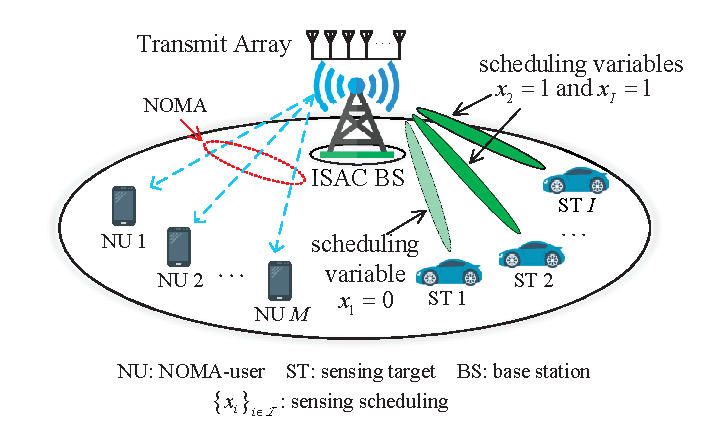
\includegraphics[width=0.9\textwidth]{figs_tvt_cld/Figure1.eps}
    \caption{An illustrative system model}
    \label{fig:figure_model}
\end{figure*}

Figure \ref{fig:figure_model} illustrates the considered NOMA-aided ISAC system. The ISAC BS is equipped with a uniform linear array of $K$-antennas providing the downlink transmission to a group of NUs via NOMA. Meanwhile, the ISAC BS also performs the radar sensing towards a group of STs. There exists $M$ single-antenna NUs denoted by $\mathcal{M}=\{1,2,...,M\}$ that are receiving data from the ISAC BS. For each NU $m\in\mathcal{M}$, we use $D_m$ to denote its required amount of data to receive. Meanwhile, there exist $I$ STs which are denoted by $\mathcal{I}=\{1,2,...,I\}$ to be sensed. In this work, we assume that the ISAC BS knows the existence of STs (e.g., their locations and directions). The ISAC BS performs radar sensing to the STs to estimate some specific information, e.g., the STs' moving velocities. 


\subsection{Communication Model}

We consider that the ISAC BS exploits NOMA to serve $M$ NUs simultaneously on the same frequency band. Specifically, the BS transmits a superimposed joint sensing and communication signal $\sum_{m\in\mathcal{M}}\mathbf{w}_ms_m$ to all NUs, where $\mathbf{w}_m\in \mathbb{C}^{K\times 1}$ are beamformers for delivering the information symbol $s_m$ to NU $m$. Since the superimposed NOMA signals is utilized for sensing the selected STs, the radar sensing signal will not influence the communication links. As a result, the signal $y_m$ received at NU $m$ can be given as
\begin{eqnarray}
	y_m=\sum_{j=1}^{M}\mathbf{g}_m^H\mathbf{w}_js_j+n_0,\forall m\in\mathcal{M},
	\label{def:yi}
\end{eqnarray}
where $\mathbf{g}_m=\beta_m\widetilde{\mathbf{g}}_m$ denotes the channel gain between the ISAC BS and NU $m$, $n_0$ denotes the circularly symmetric complex Gaussian noise, $\beta_m$ accounts for the large-scale channel fading gain of NU $m$, and $\widetilde{\mathbf{g}}_m\in \mathbb{C}^{K\times 1}$ denotes the small-scale fading channel component.


To facilitate the model of NOMA transmission, we suppose 
\begin{eqnarray}
	\beta_1\ge \beta_2\ge \cdots\ge \beta_M.
	\label{def:hi}
\end{eqnarray}
With the above ordering and the operations of SIC \cite{tvt.9722777}, the symbol $s_m$ for NU $m$ requires to be decoded at NU $n$, for $n\le m$ and $\forall m\in\mathcal{M}$, which yields the following achievable rate
\begin{eqnarray}
	R_{m(n)}=B\log_2\left(1+\frac{|\mathbf{g}_n^H\mathbf{w}_m|^2}{\sum_{j=1}^{m-1}|\mathbf{g}_n^H\mathbf{w}_j|^2+\sigma_n^2}\right).
	\label{def:Rij}
\end{eqnarray}
In eq. (\ref{def:Rij}), parameter $B$ denotes the channel bandwidth and $\sigma_n^2$ denotes the variance of the circularly symmetric complex Gaussian noise. 
Therefore, the overall achievable rate of NU $m$ is
\begin{eqnarray}
	R_{m}=\min_{\forall n\le m} \{R_{m(n)}\},\forall m\in\mathcal{M}.
	\label{def:Ri}
\end{eqnarray}



We use variable $t$ to denote the NOMA transmission duration. In particular, the NOMA transmission duration should satisfy the following constraint
\begin{eqnarray}
	t R_m \ge D_m,\forall m\in\mathcal{M},
	\label{def:Di}
\end{eqnarray}
which means that each NU $m$ should receive its required data volume $D_m$.

\subsection{Sensing Model}


The superimposed signal for all NUs is employed to sense the STs. With the beamforming, the ISAC BS sends a probing signal in the direction of the selected ST and receives the echo reflected from the ST. Specifically, with the priori information of direction $\theta_i$ of ST $i$, the power of the probing signal in direction $\theta_i$ can be given as
\begin{eqnarray}
	P_i=\mathbf{a}^H(\theta_i)\left(\sum_{m\in\mathcal{M}}\mathbf{w}_m\mathbf{w}_m^H\right)\mathbf{a}(\theta_i), \forall i\in\mathcal{I},
	\label{def:Pm}
\end{eqnarray}
where $\mathbf{a}(\theta_i)=\left[1,e^{j\frac{2\pi}{\lambda}d\sin(\theta_i)},\cdots,e^{j\frac{2\pi}{\lambda}d(K-1)\sin(\theta_i)}\right]^T$ is the transmit array steering vector for direction $\theta_i$. Parameters $d$ and $\lambda$ represent the antenna spacing and carrier wavelength, respectively.  $\sum_{m\in\mathcal{M}}\mathbf{w}_m\mathbf{w}_m^H$ denotes the covariance matrix of the transmitted signal, which affects the sensing quality.
To further measure the quality of the received echoes, we utilize the sensing estimation mutual information for each selected ST as the sensing quality metric. Specifically, with the NOMA transmission duration $t$, the sensing estimation mutual information extracted from the echoes of ST $i$ can be given as 
\begin{eqnarray}
		S_i=\frac{\delta}{2}\log_2\left(1+\frac{2t\alpha^2B^3\sigma_{proc}^2\mathbf{h}_i^HP_i\mathbf{h}_i}{\sum_{j\neq i}\mathbf{h}_j^HP_j\mathbf{h}_j+\sigma_n^2}\right), \forall i\in\mathcal{I},
	\label{def:Im}
\end{eqnarray}
where $\mathbf{h}_i=\mu_i\widetilde{\mathbf{h}}_i\in\mathbb{C}^{K\times 1}$ denotes the channel between the ISAC BS and ST $i$. Parameter $\alpha$ depends on the shape of the power spectral density of the probing signal, parameter $\delta$ denotes the radar's duty cycle and parameter $\sigma_{proc}^2$ denotes the variance of the range fluctuation process. Moreover, we introduce a group of binary sensing scheduling variables $\{x_i\}_{i\in\mathcal{I}}$ with $x_i=1$ meaning that ST $i$ is selected to be sensed during the considered NOMA transmission duration, while $x_i=0$ meaning the opposite case.

We use the following constraint to denote that for each ST, if it is selected, the corresponding sensing estimation mutual information should be no smaller than a required level $\Gamma_i^{\text{min}}$, i.e., 
\begin{eqnarray}
	S_i\ge x_i \Gamma_i^{\text{min}},\forall i\in\mathcal{I}.
	\label{Imcon}
\end{eqnarray}

When more than one ST is selected in each scheduling, the mean-squared cross-correlation $Q^{\text{ms}}$ of probing signals can be expressed as
\begin{footnotesize}
    \begin{align}
		{Q}^{\text{ms}}=
		\begin{cases}
			\frac{2}{\left({(\sum\limits_{i\in\mathcal{I}}x_i)}^2-\sum\limits_{i\in\mathcal{I}}x_i\right)}\sum\limits_{p=1}^{I-1}\sum\limits_{q=p+1}^{I}x_px_q{\left|\mathbf{a}^H(\theta_p)\left(\sum_{m\in\mathcal{M}}\mathbf{w}_m\mathbf{w}_m^H\right)\mathbf{a}(\theta_q)\right|}^2,&\text{when~} \sum\limits_{i\in\mathcal{I}}x_i>1,\\
			0,&\text{otherwise}.
		\end{cases}
		\label{def:Q}
	\end{align}
\end{footnotesize}
In eq. (3.9), the summation is normalized by the total number of different pairs of probing signals, i.e., $\frac{(\sum_{i\in\mathcal{I}}x_i)^2-\sum_{i\in\mathcal{I}}x_i}{2}$.
In particular, the value of ${Q}^{\text{ms}}$ should be no greater than a required level $\epsilon$ to guarantee the statistical performance of the adaptive sensing technique, i.e.,
\begin{eqnarray}
	{Q}^{\text{ms}}\le \epsilon.
	\label{Qcon}
\end{eqnarray}

	
\subsection{Problem Formulation}

In this chapter, we aim at maximizing the sensing efficiency (SEM) which is denoted by the number of the selected STs over the NOMA duration, while satisfying the communication quality requirement of each NU and radar sensing requirement of each selected ST. To achieve this goal, we jointly optimize the beamformers $\{\mathbf{w}_m\}_{m\in\mathcal{M}}$, the NOMA transmission duration $t$, and the sensing scheduling $\{x_i\}_{i\in\mathcal{I}}$. Our problem formulation is detailed as follows.
\begin{flalign}
	\text{(SEM):~} & \max~~ \frac{1}{t}\sum_{i\in\mathcal{I}}x_i	\nonumber\\
	\text{subject to:~}
	&
	\text{constraints~} (\ref{def:Di}), (\ref{Imcon}) \text{ and } (\ref{Qcon}), \nonumber
	\\ 
	&x_i\in\{0,1\}, \forall i\in\mathcal{I},\label{xmcon}
	\\
	&\mathbf{Tr}\left(\sum_{m\in\mathcal{M}}\mathbf{w}_m\mathbf{w}_m^H\right)\le P^{\text{max}},\label{TrPcon}
	\\
	&0< t\le T,\label{tcon}
	\\
	\text{variables:~} & {\{\mathbf{w}_m\}_{m \in {\cal M}}}, \{x_{i}\}_{i\in\mathcal{I}}, t.\nonumber
\end{flalign}
Constraint (\ref{def:Di}) ensures that each NU's communication requirement is satisfied. Constraint (\ref{Imcon}) ensures that the radar sensing requirement of each selected ST is guaranteed. Constraint (\ref{Qcon}) specifies an upper bound on the mean-square cross-correlation of the probing signals. Constraint (\ref{TrPcon}) ensures that the BS's transmitting power cannot exceed its power capacity $P^{\text{max}}$. Constraint (\ref{tcon}) ensures that the NOMA transmission duration cannot exceed a maximum latency denoted by $T$.


\section{Layered Decomposition and Proposed Algorithm} \label{chap3_sec_alg}

\subsection{Problem Reformulation}
Problem (SEM) is a mixed binary and non-convex optimization problem. Specifically, the binary sensing scheduling $\{x_i\}_{i\in\mathcal{I}}$ and the NOMA transmission duration $t$ are coupled in the objective function and constraint (\ref{Imcon}). Moreover, constraints (\ref{def:Di}) and (\ref{TrPcon}) are both non-convex. Therefore, it is challenging to solve Problem (SEM) directly. To address this difficulty, we propose a decomposition-based approach to solve this problem. The details are as follows. 


For each NU $m$, we firstly define $\mathbf{W}_m\triangleq\mathbf{w}_m\mathbf{w}_m^H$, with three constraints $\mathbf{W}_m\succeq 0$, $\mathbf{W}_m=\mathbf{W}_m^H$, and rank($\mathbf{W}_m$) = 1. In addition, for convenience of expression, we define 
\begin{equation}
V_i\triangleq \mathbf{h}_i^H\mathbf{a}^H(\theta_i)\left(\sum\limits_{m\in\mathcal{M}}\mathbf{W}_m\right)\mathbf{a}(\theta_i)\mathbf{h}_i.
\end{equation}
Then, constraint (\ref{Imcon}) can be rewritten as 
\begin{equation}
	\frac{tV_i}{\sum\limits_{j\neq i}V_j+\sigma_n^2}\ge \rho_i,\forall i\in\mathcal{I},
	\label{Imcon2}
\end{equation}
where
\begin{equation} \rho_i=\frac{1}{2\alpha^2B^3\sigma_{proc}^2}(2^\frac{2x_i\Gamma_i^{\text{min}}}{\delta}-1),\forall i\in\mathcal{I}.
	\label{rho}
\end{equation}
Meanwhile, constraint (\ref{Qcon}) can be rewritten as 
\begin{footnotesize}
    \begin{align}
		\frac{2}{\left({(\sum\limits_{i\in\mathcal{I}}x_i)}^2-\sum\limits_{i\in\mathcal{I}}x_i\right)}\sum\limits_{p=1}^{I-1}\sum\limits_{q=p+1}^{I}x_px_q|\mathbf{a}^H(\theta_p)\left(\sum_{m\in\mathcal{M}}\mathbf{W}_m\right)\mathbf{a}(\theta_q)|^2\le \epsilon,~~\text{when~} \sum_{i\in\mathcal{I}}x_i>1.
		\label{Qcon2}
	\end{align}
\end{footnotesize}
Thus, Problem (SEM) can be equivalently transformed into \setcounter{equation}{17}
\begin{flalign}
	\text{(SEM-E):~} & \max~~ \frac{1}{t}\sum_{i\in\mathcal{I}}x_i	\nonumber\\
	\text{subject to:~}
	&
	\text{constraints~} (\ref{def:Di}), (\ref{xmcon}), (\ref{tcon}), (\ref{Imcon2}) \text{ and } (\ref{Qcon2}),\nonumber
	\\ 
	&\mathbf{Tr}\left(\sum_{m\in\mathcal{M}}\mathbf{W}_m\right)\le P^{\text{max}},\label{TrPcon1}
	\\
	&\mathbf{W}_m\succeq 0, \forall m, \label{addcon1}
	\\
	&\mathbf{W}_m=\mathbf{W}_m^H, \forall m, \label{addcon2}
	\\
	&\text{rank}(\mathbf{W}_m)=1, \forall m, \label{addcon3}
	\\
	\text{variables:~} & {\{\mathbf{W}_m\}_{m \in {\cal M}}}, \{x_{i}\}_{i\in\mathcal{I}}, t.\nonumber
\end{flalign}

\subsection{Decomposition of Problem (SEM-E)}

To address the difficulty due to the mixed binary and non-convexity, we propose a vertical decomposition as follows.



 

\begin{figure*}
	\centering
	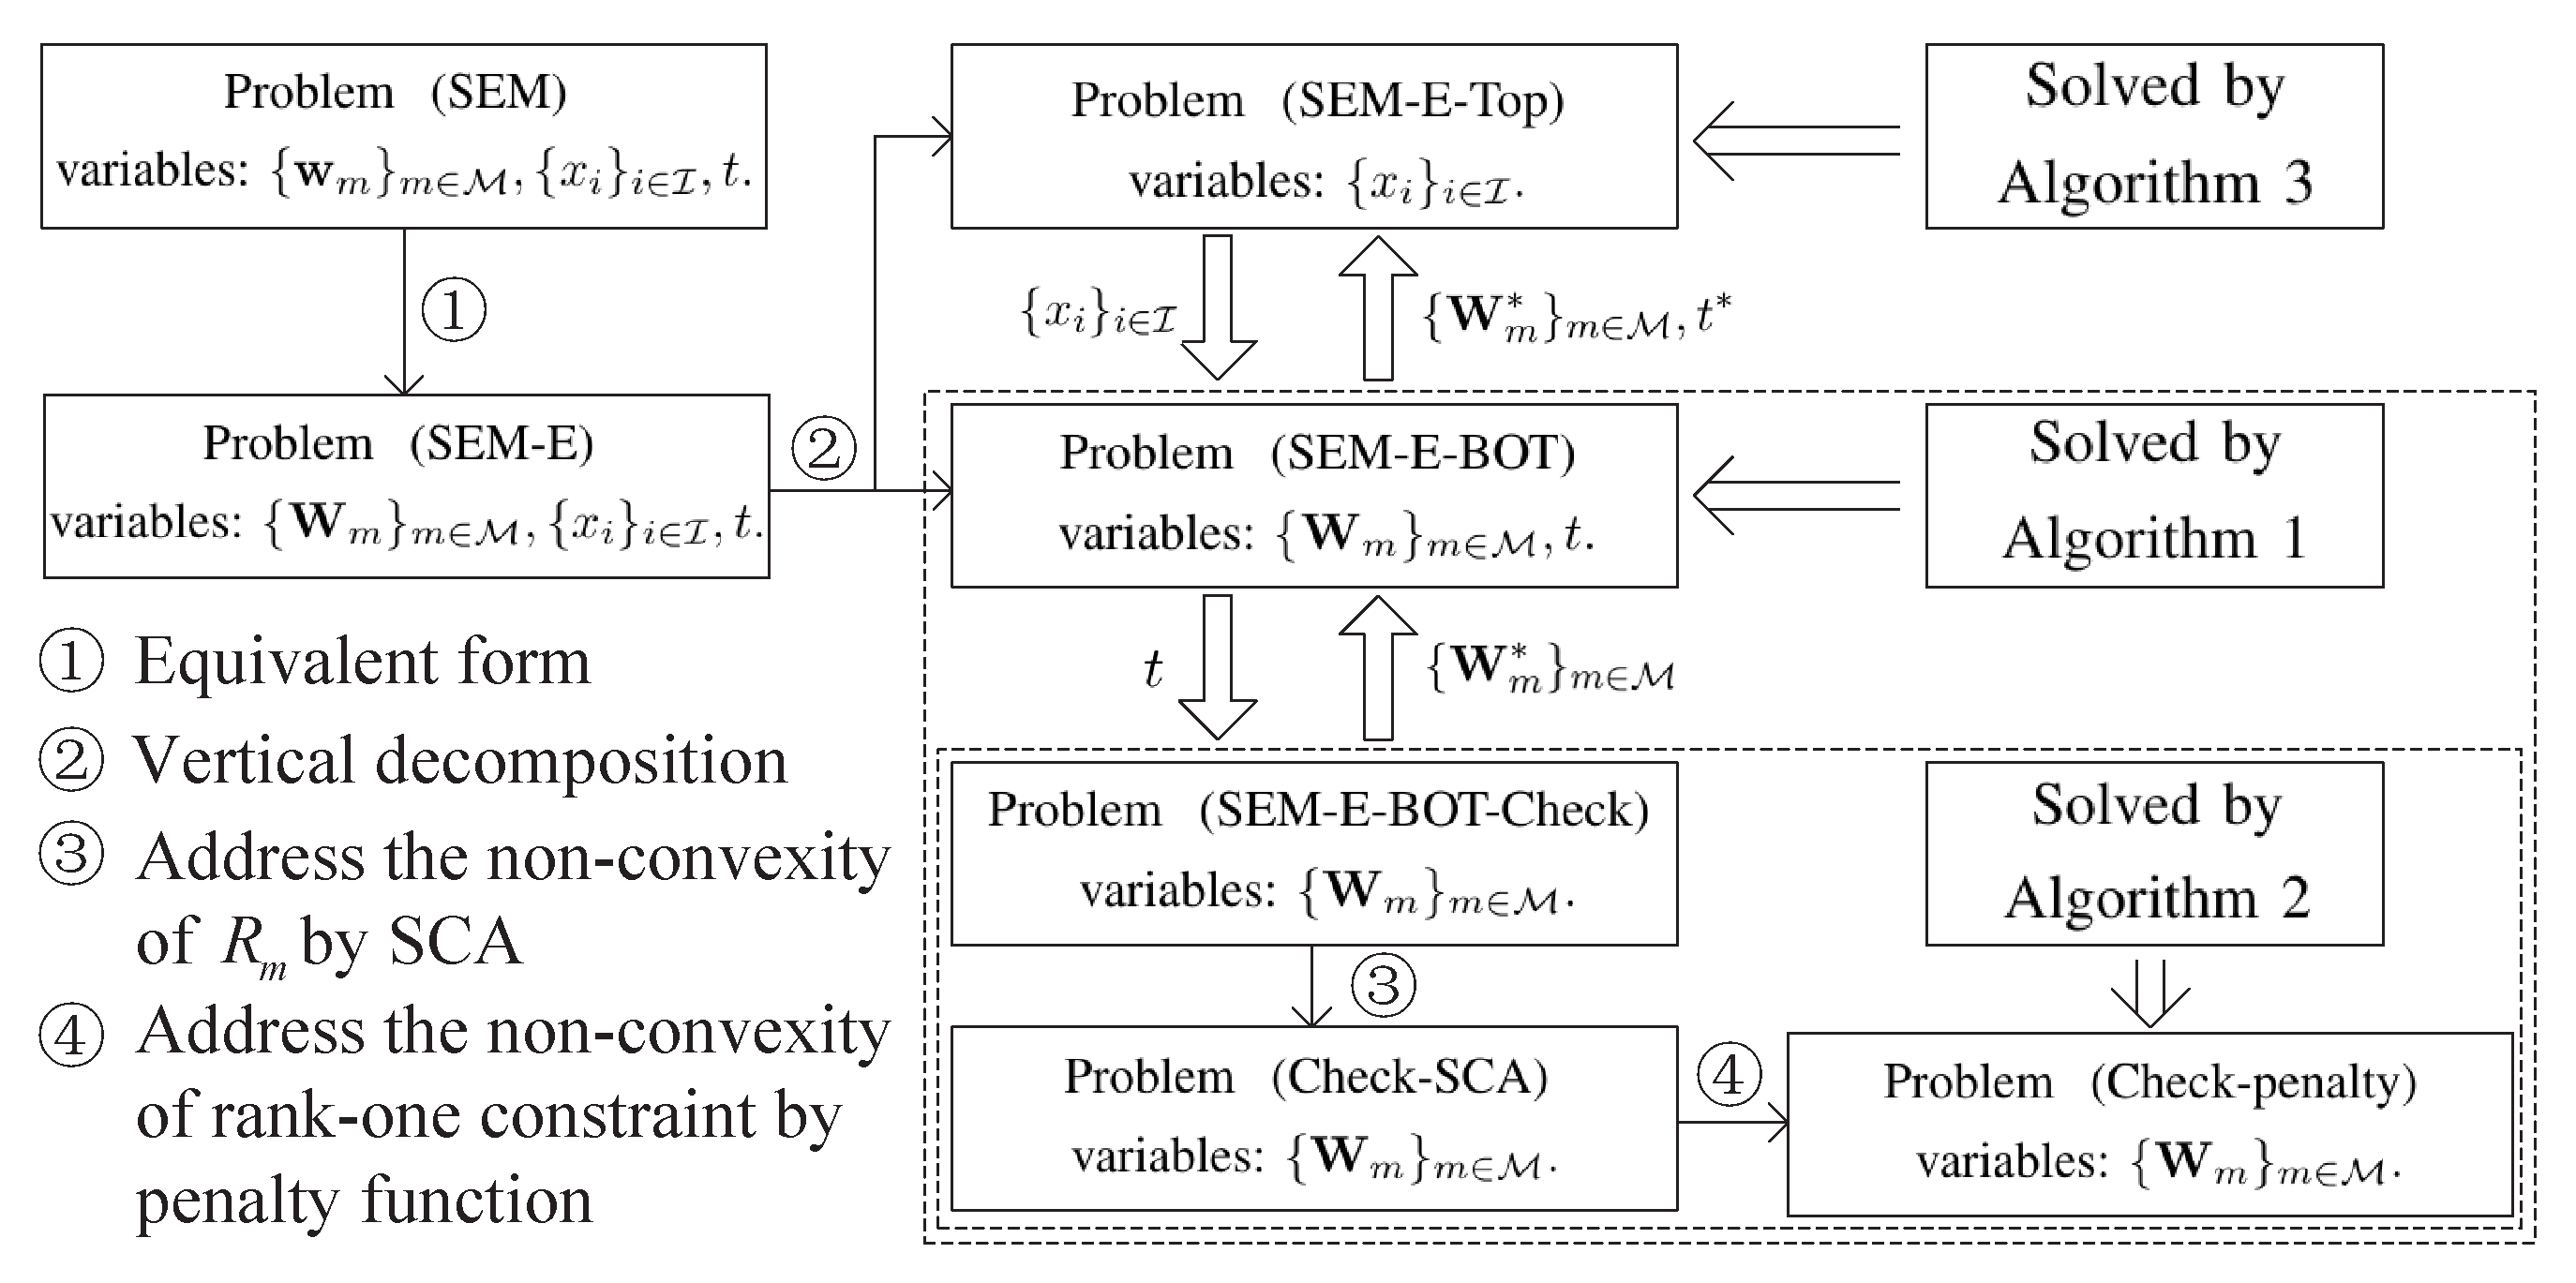
\includegraphics[width=0.9\textwidth]{figs_tvt_cld/Figure2.eps}
	\caption{Decomposition of Problem (SEM-E)}
	\label{fig:decomposion}
\end{figure*}




\subsubsection{Bottom-problem under given $\{x_i\}_{i\in\mathcal{I}}$}
Given the sensing scheduling $\{x_i\}_{i\in\mathcal{I}}$, Problem (SEM-E) turns into the following bottom-problem.
\begin{flalign}
	\text{(SEM-E-BOT):~} & E^{\text{BOT}}(\{x_i\}_{i\in\mathcal{I}})=\max~~ \frac{1}{t}\sum_{i\in\mathcal{I}}x_i \nonumber\\
	\text{subject to:~}
	&
	\text{constraints~} (\ref{def:Di}), (\ref{tcon}), (\ref{Imcon2}), (\ref{Qcon2}), (\ref{TrPcon1}), (\ref{addcon1}), (\ref{addcon2})\nonumber
	\\
	&~~~~~~~~~~~~~~~~~~ \text{ and } (\ref{addcon3}),\nonumber
	\\
	\text{variables:~} & {\{\mathbf{W}_m\}_{m \in {\cal M}}}, t.\nonumber
\end{flalign}




\subsubsection{Top-problem of optimizing $\{x_i\}_{i\in\mathcal{I}}$}
After solving Problem (SEM-E-BOT) and obtaining the value of $E^{\text{BOT}}(\{x_i\}_{i\in\mathcal{I}})$ with the given $\{x_i\}_{i\in\mathcal{I}}$, we then optimize $\{x_i\}_{i\in\mathcal{I}}$, which results in the following optimization problem.
\begin{flalign}
	\text{(SEM-E-Top):~} &
	\max~~E^{\text{BOT}}(\{x_i\}_{i\in\mathcal{I}}) \nonumber
	\\
	\text{subject to:~}
	&
	\text{constraint~} (\ref{xmcon}),  \nonumber
	\\
	\text{variables:~} & {\{x_i\}_{i\in\mathcal{I}}}. \nonumber
\end{flalign}

As shown in Figure \ref{fig:decomposion}, the above top-problem and bottom-problem work in a master-slave manner, i.e., for each $\{x_i\}_{i\in\mathcal{I}}$ given by Problem (SEM-E-Top), we invoke the subroutine for solving Problem (SEM-E-BOT) and return the result to Problem (SEM-E-Top).
		
		
		
\subsection{Proposed Algorithm for Solving Problem (SEM-E-BOT)}
Under a given $\{x_i\}_{i\in\mathcal{I}}$, Problem (SEM-E-BOT) can be considered as a problem of finding the minimum $t$ that can ensure the feasible region specified by constraints (\ref{def:Di}), (\ref{Imcon2}) and (\ref{Qcon2})-(\ref{addcon3}) is non-empty. To this end, we formulate an optimization problem, which is used to check whether constraints (\ref{def:Di}), (\ref{Imcon2}) and (\ref{Qcon2})-(\ref{addcon3}) can form a non-empty set or not under a given $t$, as follows.
\begin{flalign}
	\text{(SEM-E-BOT-Check):~} & O_{(t)}=\min~~ \mathbf{Tr}\left(\sum_{m\in\mathcal{M}}\mathbf{W}_m\right)-P^{\text{max}} \nonumber\\
	\text{subject to:~}
	&R_m\ge\frac{D_m}{t},\forall m,\label{check1}
	\\
	&V_i\ge \frac{\rho_i}{t}\left(\sum_{j\neq i}V_j+\sigma_n^2\right),\forall i,\label{check2}
	\\
	&\text{constraints~}  (\ref{Qcon2}), (\ref{addcon1}), (\ref{addcon2}) \text{ and } (\ref{addcon3}),\nonumber
	\\
	\text{variables:~} & {\{\mathbf{W}_m\}_{m \in {\cal M}}}.\nonumber
\end{flalign}
Recall that constraints (\ref{check1}) and (\ref{check2}) are the equivalent form of constraints (\ref{def:Di}) and (\ref{Imcon2}), respectively, when the value of $t$ is given. Moreover, regarding constraint (\ref{check2}), it is noticed that for each ST $i$, if $x_i=0$, constraint (\ref{check2}) can always be guaranteed according to the definitions of $V_i$ in eq. (14) and $\rho_i$ in eq. (\ref{rho}). Specifically, if the optimal output $O_{(t)}\le 0$, then the feasible region specified by constraints (\ref{def:Di}), (\ref{Imcon2}) and (\ref{Qcon2})-(\ref{addcon3}) is non-empty, meaning that Problem (SEM-E-BOT) is feasible under the given $t$. Otherwise (i.e., $O_{(t)}>0$), Problem (SEM-E-BOT) is infeasible. In addition, we identify the following feature.



\begin{proposition}
	\label{proposition:feature1}
	The value of $O_{(t)}$ of Problem (SEM-E-BOT-Check) is non-increasing in $t$.
\end{proposition}
\begin{proof}
	It can be observed that the feasible region constructed by constraints (\ref{Qcon2}), (\ref{addcon1})-(\ref{check2}) increases, when $t$ increases. Consequently, the minimum value of the objective function (i.e., $O_{(t)}$) is non-increasing in $t$.
\end{proof}


By leveraging Proposition \ref{proposition:feature1}, we can perform a bisection-search on $t\in(0,T]$ to solve Problem (SEM-E-BOT) and obtain the value of $E^{\text{BOT}}(\{x_i\}_{i\in\mathcal{I}})$. Specifically, if the currently given $t$ leads $O_{(t)}\le 0$, we reduce $t$. Otherwise, we increase $t$. Based on the above idea, we propose an efficient bisection-search based algorithm to solve Problem (SEM-E-BOT). The detail is shown in Algorithm 4.

\begin{algorithm}
	\caption{: To solve Problem (SEM-E-BOT) and obtain $E^{\text{BOT}}(\{x_i\}_{i\in\mathcal{I}})$}
	\begin{algorithmic}[1]
		\STATE  \textbf{Initialization:} Set the convergence accuracy for the bisection-search $\vartheta$ as a very small number. Set $t^{\text{upp}}=T$ and $t^{\text{low}}=0$.
		\WHILE  {$|t^{\text{upp}}-t^{\text{low}}|>\vartheta$}
		\STATE  Set $t^{\text{cur}}=\frac{t^{\text{upp}}+t^{\text{low}}}{2}$.
		\STATE  Given $t^{\text{cur}}$, use Subroutine-O to calculate $O_{(t)}$.
		\IF {$O_{(t)}\le 0$}
		\STATE  Set $t^{\text{upp}}=t^{\text{cur}}$.
		\ELSE
		\STATE  Set $t^{\text{low}}=t^{\text{cur}}$.
		\ENDIF
		\ENDWHILE
		\STATE \textbf{Output:} $E^{\text{BOT}}(\{x_i\}_{i\in\mathcal{I}})=\frac{1}{t^{\text{cur}}}\sum_{i\in\mathcal{I}}x_i$
		\end{algorithmic}
\end{algorithm}

Notice that in Step 4 of Algorithm 4, a subroutine-O is required to calculate the value of $O_{(t)}$, the details of which are shown in the next subsection.

\subsection{Proposed Subroutine-O for Calculating $O_{(t)}$}


To solve Problem (SEM-E-BOT-Check) and obtain the value of $O_{(t)}$, there are two difficulties lie in the non-convexity of constraints (\ref{addcon3}) and (\ref{check1}). To propose a subroutine, we first do the following operations. With eq. (\ref{def:Ri}), constraint (\ref{check1}) can be rewritten as 
\begin{eqnarray}
	R_{m(n)}\ge\frac{D_m}{t}, \forall m\in\mathcal{M}, n\le m.
	\label{def:Ri_re}
\end{eqnarray}
We define $\mathbf{G}_m\triangleq\mathbf{g}_m\mathbf{g}_m^H$ and rewrite constraint (\ref{def:Ri_re}) as
\begin{equation}
	\begin{split}
		R_{m(n)}&=B\log_2\left(\sigma_n^2+\sum_{j=1}^{m}\mathbf{Tr}\left(\mathbf{G}_n\mathbf{W}_j\right)\right)\\&~~~~-B\log_2\left(\sigma_n^2+\sum_{j=1}^{m-1}\mathbf{Tr}\left(\mathbf{G}_n\mathbf{W}_j\right)\right)\ge\frac{D_m}{t}, \forall m\in\mathcal{M}, n\le m.
		\label{def:Rij_re}
	\end{split}
\end{equation}
Constraint (\ref{def:Ri_re}) is non-convex due to the second term of $R_{m(n)}$. To tackle this difficulty, we adopt the operations of SCA. Specifically, we first define 
\begin{equation}
	L_{m(n)}\hspace{-0.1cm}\triangleq\hspace{-0.1cm}-B\log_2\hspace{-0.1cm}\left(\sigma_n^2+\sum_{j=1}^{m-1}\mathbf{Tr}\left(\mathbf{G}_n\mathbf{W}_j\right)\right)\hspace{-0.1cm},\forall m\in\mathcal{M}, n\le m.
\end{equation}
Then, we utilize the first-order Taylor expansion of $\{\mathbf{W}_m\}_{m\in\mathcal{M}}$ for any given local point $\left(\mathbf{W}_1^u,\cdots,\mathbf{W}_M^u\right)$ in the feasible domain in the $u$-th iteration as its lower bound, i.e.,
\begin{equation}
	\begin{split}
		L_{m(n)}\ge L_{m(n)}^{\text{lb}}\triangleq& -B\log_2\left(\sigma_n^2+\sum_{j=1}^{m-1}\mathbf{Tr}\left(\mathbf{G}_n\mathbf{W}_j^u\right)\right)\\&-B\frac{\sum_{j=1}^{m-1}\mathbf{Tr}\left(\mathbf{G}_n\left(\mathbf{W}_j-\mathbf{W}_j^u\right)\right)}{\left(\sigma_n^2+\sum_{j=1}^{m-1}\mathbf{Tr}\left(\mathbf{G}_n\mathbf{W}_j^u\right)\right)\ln2}, \forall m\in\mathcal{M}, n\le m.
		\label{def:Fij_re}
	\end{split}
\end{equation}
Based on $L_{m(n)}^{\text{lb}}$, we define the lower bound of $R_{m(n)}$ as
\begin{eqnarray}
	R_{m(n)}^{\text{lb}}\triangleq B\log_2\left(\sigma_n^2+\sum_{j=1}^{m}\mathbf{Tr}\left(\mathbf{G}_n\mathbf{W}_j\right)\right)+L_{m(n)}^{\text{lb}}\ge\frac{D_m}{t}, \forall m\in\mathcal{M}, n\le m.
	\label{def:Rijlb_re}
\end{eqnarray}
By using $R_{m(n)}^{\text{lb}}$ to replace $R_{m(n)}$, we can transform constraint (\ref{def:Rij_re}) into a convex one as constraint (\ref{def:Rijlb_re}).

After the above operations, Problem (SEM-E-BOT-Check) can be rewritten as
\begin{flalign}
	\text{(Check-SCA):~} & O_{(t)}=\min~~ \mathbf{Tr}\left(\sum_{m\in\mathcal{M}}\mathbf{W}_m\right)-P^{\text{max}} \nonumber\\
	\text{subject to:~}
	&\text{constraints~}  (\ref{Qcon2}), (\ref{addcon1}), (\ref{addcon2}), (\ref{addcon3}), (\ref{check2}) \text{ and } (\ref{def:Rijlb_re}), \nonumber
	\\
	\text{variables:~} & {\{\mathbf{W}_m\}_{m \in {\cal M}}}.\nonumber
\end{flalign}
With this optimization problem, the remaining difficulty comes from the non-convexity of the rank-one constraint (\ref{addcon3}). To tackle this issue, we adopt the penalty-based algorithm \cite{tvt.nocedal1999numerical}. Specifically, since matrix $\mathbf{W}_m$ is positive semi-definite according to constraint (\ref{addcon1}), all the eigenvalues of $\mathbf{W}_m$ are non-negative, i.e., $\lambda_k\left(\mathbf{W}_m\right)\ge 0,\forall m,k=1,2,...,K$, where $\lambda_k(\cdot)$ represents the $k$-th eigenvalue of a matrix. Due to $\mathbf{Tr}\left(\mathbf{W}_m\right)=\sum_{k=1}^{K}\lambda_k\left(\mathbf{W}_m\right)$, we first transform the rank-one constraint (\ref{addcon3}) into an equivalent equality constraint
\begin{eqnarray}
	\mathbf{Tr}\left(\mathbf{W}_m\right)-\lambda_{\max}\left(\mathbf{W}_m\right)=0,\forall m\in\mathcal{M},
	\label{penaltycon}
\end{eqnarray}
where $\lambda_{\max}(\cdot)$ denotes the maximum eigenvalue of a matrix. Therefore, eq. (\ref{penaltycon}) holds when matrix $\mathbf{W}_m$ is a rank-one matrix. On the contrary, since $\mathbf{W}_m$ is positive semi-definite, we derive that the trace of the matrix is greater than the maximum eigenvalue of the matrix, i.e., $\mathbf{Tr}\left(\mathbf{W}_m\right)-\lambda_{\max}\left(\mathbf{W}_m\right)>0$. In order to obtain a rank-one matrix, we drop the rank-one constraint (\ref{addcon3}) and introduce a penalty term into the objective function, which results in the following new objective function
\begin{eqnarray}
		\min~~ \mathbf{Tr}\left(\sum_{m\in\mathcal{M}}\mathbf{W}_m\right)-P^{\text{max}}+\eta\sum_{m\in\mathcal{M}}\left(\mathbf{Tr}\left(\mathbf{W}_m\right)-\lambda_{\max}\left(\mathbf{W}_m\right)\right),
	\label{newobj}
\end{eqnarray}
where $\eta>0$ is the penalty factor. However, the second term of the penalty term makes the objective function non-convex. By further exploiting SCA, we can transform (\ref{newobj}) into a convex one. Specifically, by exploiting the first-order Taylor expansion at the feasible point $\left(\mathbf{W}_1^u,\cdots,\mathbf{W}_M^u\right)$ at the $u$-th iteration, the upper bound of the penalty term is given in
\begin{eqnarray}
	\begin{split}
	&\mathbf{Tr}\left(\mathbf{W}_m\right)-\lambda_{\max}(\mathbf{W}_m^{u})-\left({\mathbf{z}_{m,\max}^u}\right)^H\left(\mathbf{W}_m-\mathbf{W}_m^{u}\right)\mathbf{z}_{m,\max}^u\\&\ge\mathbf{Tr}\left(\mathbf{W}_m\right)-\lambda_{\max}\left(\mathbf{W}_m\right)\ge 0,
	\label{SCApenalty}
	\end{split}
\end{eqnarray} 
where $\mathbf{z}_{m,\max}$ is the unit eigenvector with respect to the maximum eigenvalue $\lambda_{\max}\left(\mathbf{W}_i\right)$. Thus, we derive the iterative optimization Problem (Check-penalty) as follows, which is Problem (Check-SCA) in the $(u+1)$-th iteration.
\begin{flalign}
		\text{(Check-penalty):~} & \min \mathbf{Tr}\left(\sum_{m\in\mathcal{M}}\mathbf{W}_m\right)-P^{\text{max}}\nonumber\\&\hspace{-2cm}+\eta\sum_{m\in\mathcal{M}}\left(\mathbf{Tr}\left(\mathbf{W}_m\right)-\lambda_{\max}(\mathbf{W}_m^{u})-\left({\mathbf{z}_{m,\max}^u}\right)^H\left(\mathbf{W}_m-\mathbf{W}_m^{u}\right)\mathbf{z}_{m,\max}^u\right) \nonumber\\
		\text{subject to:~}&
		\text{constraints~}  (\ref{Qcon2}), (\ref{addcon1}), (\ref{addcon2}),  (\ref{check2})  \text{ and } (\ref{def:Rijlb_re}) ,\nonumber
		\\
		\text{variables:~}&  {\{\mathbf{W}_m\}_{m \in {\cal M}}}.\nonumber
\end{flalign}




\begin{proposition}
	\label{proposition:feature2}
	Problem (Check-penalty) is a strictly convex optimization with $\{\mathbf{W}_m\}$.
\end{proposition}
\begin{proof}
	It can be identified that the objective function in Problem (Check-penalty) is strictly convex with  $\{\mathbf{W}_m\}_{m\in\mathcal{M}}$. Constraints (\ref{addcon1}) and (\ref{addcon2}) result in a convex feasible set for $\{\mathbf{W}_m\}_{m\in\mathcal{M}}$. It can also be identified that constraints (\ref{Qcon2}) and (\ref{def:Rijlb_re}) are convex with $\{\mathbf{W}_m\}_{m\in\mathcal{M}}$, and constraint (\ref{check2}) is affine. Therefore, it can be concluded that Problem (Check-penalty) is a convex optimization problem with $\{\mathbf{W}_m\}_{m\in\mathcal{M}}$.
\end{proof}



Based on Proposition 6, Problem (Check-penalty) can be solved efficiently with several existing solvers for convex optimizations, e.g., CVX, in an iterative way. After convergence, i.e., when $\mathbf{Tr}(\mathbf{W}_m)$ is equal to $\lambda_{\max}(\mathbf{W}_m)$, we can derive that \setcounter{equation}{31}
\begin{eqnarray}
	\mathbf{W}_m=\lambda_{\max}\left(\mathbf{W}_m\right)\mathbf{z}_{m,\max}(\mathbf{z}_{m,\max})^H,\forall m\in\mathcal{M}.
	\label{recovery1}
\end{eqnarray}
Accordingly, we can calculate the optimal beamformer $\mathbf{w}_m$ according to the following equation
\begin{eqnarray}
	\mathbf{w}_m^*=\sqrt{\lambda_{\max}\left(\mathbf{W}_m\right)}\mathbf{z}_{m,\max},\forall m\in\mathcal{M}.
	\label{recovery2}
\end{eqnarray}
In summary, the detail of the proposed penalty-based algorithm (i.e., Subroutine-O) is shown in Algorithm 5, which is explained as follows.
\subsubsection{Step 4 to Step 7} For the current value of penalty factor $\eta$, we can obtain the solution for the convergence of $\mathbf{W}_m$ by CVX in an iterative solution. The $\mathbf{W}_m$ converges under the value of this penalty factor $\eta$ when the change of $\mathbf{W}_m$ falls below the threshold $\Delta$.
\subsubsection{Step 2 to Step 10} In Step 9, we check whether the value of the penalty term falls below the threshold $\Delta$. If yes, the iteration is terminated. Otherwise, we increase the value of penalty factor to decrease the penalty term in the next iteration. In particular, we set the initial value of the next round iteration to the convergent value of the previous round iteration in Step 8, which provides a starting point to reduce the number of iterations in the next round iteration.
\subsubsection{Step 11} When the algorithm converges, the approximate optimal beamformer $\mathbf{w}_m$ can be obtained by eq. (\ref{recovery2}). Meanwhile, we can obtain the value of $O_{(t)}$ which is used by Algorithm 4 to update the value of $t$.

\begin{algorithm}
	\caption{: Subroutine-O to calculate the value of $O_{(t)}$ and $\mathbf{w}_m^*$.}
	\begin{algorithmic}[1]
		\STATE  \textbf{Initialization:} Set $\mathbf{w}_m^0=\sqrt{\frac{P^{\text{max}}}{N}}\left[1,0,...,0\right]^T$. Set $\mathbf{W}_m^0=\mathbf{w}_m^0(\mathbf{w}_m^0)^H$. Initialize a proper penalty factor $\eta$, a proper coefficient $c>1$ and a proper maximum number of iterations $U^{\text{max}}$. Set the convergence accuracy $\Delta$ as a very small number.
		\REPEAT  
		\STATE  Set iteration number $u=0$. 
		\REPEAT
		\STATE  Solve Problem (Check-penalty) with $\mathbf{W}_m^u$ by CVX, then obtain $\mathbf{W}_m^{u+1}$.
		\STATE  Update $u=u+1$.
		\UNTIL  {$|\mathbf{W}_m^{u+1}-\mathbf{W}_m^u|<\Delta$ \textbf{or} $u> U^{\text{max}}$}  
		\STATE  Update $\mathbf{W}_m^{0}=\mathbf{W}_m^{u}$.
		\STATE  Increase the penalty factor with $\eta=c\eta$.
		\UNTIL  {$\sum_{m\in\mathcal{M}}|\mathbf{Tr}\left(\mathbf{W}_m^u\right)-\lambda_{\max}\left(\mathbf{W}_m^u\right)|<\Delta$}
		\STATE \textbf{Output:} Obtain $\mathbf{w}_m^*$ according to (\ref{recovery2}). Obtain $O_{(t)}= \mathbf{Tr}\left(\sum_{m\in\mathcal{M}}\mathbf{W}_m^*\right)-P^{\text{max}}$.
	\end{algorithmic}
\end{algorithm}




	


\subsection{Proposed Algorithm for Solving Problem (SEM-E-Top)}

With Algorithm 4 (and its Subroutine-O), for given $\{x_i\}_{i\in\mathcal{I}}$, we can solve Problem (SEM-E-BOT) and calculate the value $E^{\text{BOT}}(\{x_i\}_{i\in\mathcal{I}})$. We thus proceed to solve Problem (SEM-E-Top), i.e., to find the optimal sensing scheduling $\{x_i\}_{i\in\mathcal{I}}$ that can maximize the sensing efficiency. The difficulty of solving Problem (SEM-E-Top) lies in that we cannot express $E^{\text{BOT}}(\{x_i\}_{i\in\mathcal{I}})$ in an analytical way. To tackle this difficulty, we adopt a CE learning based algorithm to optimize the sensing schedule variables $\{x_i\}_{i\in\mathcal{I}}$ \cite{tvt.de2005tutorial}. The key of the CE learning is to update the probability of the value since the sensing scheduling is a group of binary variables. Specifically, we virtually model $\{x_i\}_{i\in\mathcal{I}}$ as random variables, with each $x_i$ following a Bernoulli distribution of parameter $\omega_i$ as follows: 
\begin{eqnarray}
	\Phi_i(x_i)={\omega_i}^{x_i}{(1-\omega_i)}^{(1-x_i)},\forall i\in\mathcal{I}.
	\label{Bernoulli}
\end{eqnarray}
Then, we will update $\Phi_i(x_i)$ in each iteration until we reach the sensing scheduling that can maximize the sensing efficiency. The details include the following three steps \cite{tvt.de2005tutorial}:
\begin{itemize}
	\item Randomly generate a batch of samples with each sample denoting a $1\times I$ vector. Specifically, the $i$-th element of each sample follows the distribution of $\Phi_i(x_i)$ in eq. (\ref{Bernoulli}).
	\item Select a portion of the elite samples from the batch based on the results corresponding to each sample.
	\item Update $\{\omega_i\}_{i\in\mathcal{I}}$ based on the CE learning criterion.
\end{itemize}
In particular, different from the conventional CE algorithm, we propose a new strategy for updating probabilities based on the memory set that accelerate the convergence of the algorithm. The details are shown in Algorithm 6 and explained as follows.
\subsubsection{Step 3} Given the current $\{\omega_i\}_{i\in\mathcal{I}}$, we generate a batch of $F$ samples $\{\mathbf{x}^f\}_{f=1,2,...,F}$, where the superscript $f$ is the index of the samples. Specifically, each $\mathbf{x}^f$ denotes the $f$-th sample $\{x_i\}_{i\in\mathcal{I}}$ with $x_i=0$ or $x_i=1$, which are randomly generated according to the current $\{\omega_i\}_{i\in\mathcal{I}}$.
\subsubsection{Step 4 to Step 12} Given the sample of $\mathbf{x}^f$, we can obtain a group of samples of $\{x_i\}_{i\in\mathcal{I}}$. By invoking Algorithm 4, we can obtain the value of the sensing efficiency corresponding to each sample of $\mathbf{x}^f$, i.e., $E^{\text{BOT}}(\{x_i\}^f_{i\in\mathcal{I}})$. In particular, in Step 9, we store the generated sample values and the corresponding results in the sample memory set (SMS) and the value memory set (VMS), respectively. When the subsequent randomly generated samples already exist in the (SMS), we can directly obtain the corresponding values from the (VMS) without invoking Algorithm 4, which thus save the computational time. In Step 12, the samples of $\{\mathbf{x}^f\}_{f=1,2,...,F}$ are reordered from the largest to the smallest according to the values of the obtained sensing efficiency.
\subsubsection{Step 13 to Step 17} Based on the CE criterion, we can update $\{\omega_i\}_{i\in\mathcal{I}}$ according to the following function:
\begin{eqnarray}
	\omega_i^*=\arg\max_{0\le\omega_i\le 1}\mathbb{E}\left[\Phi_i(x_i)\right],\forall i\in\mathcal{I},
	\label{update1}
\end{eqnarray}
where $\mathbb{E}\left[\cdot\right]$ represents the expectation of $\Phi_i(x_i)$ of the samples selected. By selecting the best $\hat{F}$ samples in each iteration, eq. (35) can be equivalent to the following equation:
\begin{eqnarray}
	\omega_i^*=\frac{1}{\hat{F}}\sum_{f=1}^{\hat{F}}x_i^f,\forall i\in\mathcal{I}.
	\label{update2}
\end{eqnarray}
\begin{algorithm}
	\caption{: CE learning based algorithm for solving Problem (SEM-E-Top) and obtaining $\{x_i^*\}_{i\in\mathcal{I}}$.}
	\begin{algorithmic}[1]
		\STATE  \textbf{Initialization:} Initialize $\omega_i=0.5,\forall i\in\mathcal{I}$, and set $\Lambda$ as a very small positive number. Set sample memory set $\text{SMS}=\varnothing$, value memory set $\text{VMS}=\varnothing$.
		\WHILE {1}
		\STATE Randomly generate a batch of $F$ binary samples $\{\mathbf{x}^f\}_{f=1,2,...,F}$ of $I$ length according to the current $\{\omega_i\}_{i\in\mathcal{I}}$. Each $\mathbf{x}^f$ denotes the $f$-th sample $\{x_i\}_{i\in\mathcal{I}}$ with $x_i=0$ or $1$.
		\FOR {each $\mathbf{x}^f\in\{\mathbf{x}^f\}_{f=1,2,...,F}$}
		\IF {$x^f\in\text{SMS}$}
		\STATE Obtain the corresponding $E^{\text{BOT}}(\{x_i\}^f_{i\in\mathcal{I}})$ from the $\text{VMS}$.
		\ELSE
		\STATE For the current $\{x_i\}_{i\in\mathcal{I}}$, invoke Algorithm 4 to obtain the value of $E^{\text{BOT}}(\{x_i\}^f_{i\in\mathcal{I}})$.
		\STATE Store current $\{x_i\}_{i\in\mathcal{I}}$ in $\text{SMS}$ and $E^{\text{BOT}}(\{x_i\}^f_{i\in\mathcal{I}})$ in $\text{VMS}$.
		\ENDIF
		\ENDFOR
		\STATE Reorder the samples $\{\mathbf{x}^f\}_{f=1,2,...,F}$ in the order of $E^{\text{BOT}}(\{x_i\}^f_{i\in\mathcal{I}})$ from the largest to the smallest.
		\STATE Select $\hat{F}$ best samples from the reordered samples in order, use eq. (\ref{update2}) to calculate $\{\omega_i^*\}_{i\in\mathcal{I}}$, use eq. (\ref{update3}) to calculate $\{\omega_i^{*,\text{glo}}\}_{i\in\mathcal{I}}$ and further update $\{\omega_i^{\text{upd}}\}_{i\in\mathcal{I}}$ with eq. (\ref{update4}).
		\IF {$\max_{i\in\mathcal{I}}|\omega_i^{\text{upd}}-\omega_i|<\Lambda$}
		\STATE \textbf{break}
		\ENDIF
		\STATE Set $\omega_i=\omega_i^{\text{upd}},\forall i\in\mathcal{I}$.
		\ENDWHILE
		\STATE Set $E^*=\max E^{\text{BOT}}(\{x_i\}^f_{i\in\mathcal{I}})$, $\{x_i^*\}_{i\in\mathcal{I}}=\arg\max E^{\text{BOT}}(\{x_i\}^f_{i\in\mathcal{I}})$.
		\STATE \textbf{Output:} the tuple of the solutions $(E^*,\{x_i^*\}_{i\in\mathcal{I}})$.
	\end{algorithmic}
\end{algorithm}
In particular, to improve the convergence rate, we introduce a global optimum parameter $\omega_i^{*,\text{glo}}$. By selecting the best $\tilde{F}$ samples in the corresponding SMS based on the values in the VMS, $\omega_i^{*,\text{glo}}$ can be given as
\begin{eqnarray}
	\omega_i^{*,\text{glo}}=\frac{1}{\tilde{F}}\sum_{f=1}^{\tilde{F}}x_i^f,\forall i\in\mathcal{I}.
	\label{update3}
\end{eqnarray}
Finally, the next iteration of $\{\omega_i\}_{i\in\mathcal{I}}$ is updated according to the following equation:
\begin{eqnarray}
	\omega_i^{\text{upd}}=\kappa_1\omega_i+\kappa_2\omega_i^*+\kappa_3\omega_i^{*,\text{glo}},\forall i\in\mathcal{I},
	\label{update4}
\end{eqnarray}
where parameters $\kappa_1$, $\kappa_2$ and $\kappa_3$ are the weight factors with $\kappa_1+\kappa_2+\kappa_3=1$. Algorithm 6 terminates when the change in $\{\omega_i\}_{i\in\mathcal{I}}$ falls below the threshold $\Lambda$.

These three algorithms are executed in a master-slave manner (i.e., Algorithm 6 invokes Algorithm 4 and Algorithm 4 further invokes Algorithm 5), which solves the original sensing-efficiency optimization problem.





\section{Numerical Results} \label{chap3_sec_result}

\begin{figure*}
	\centering
	\subfigure[t=0.8 ms]{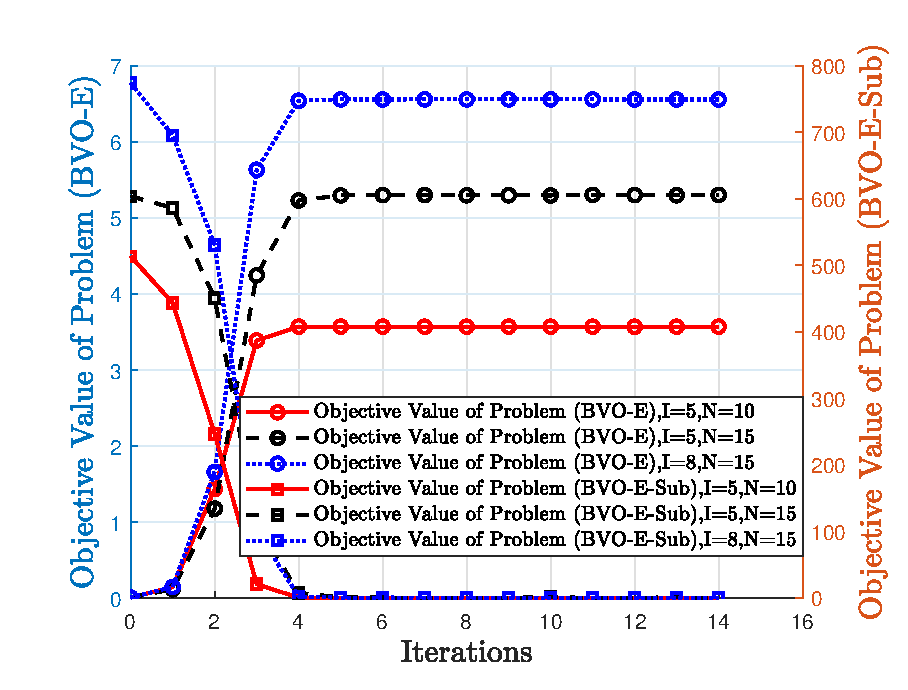
\includegraphics[width=0.6\textwidth]{figs_tvt_cld/Figure3a.eps}\label{4-1}}
	\subfigure[t=1.07 ms]{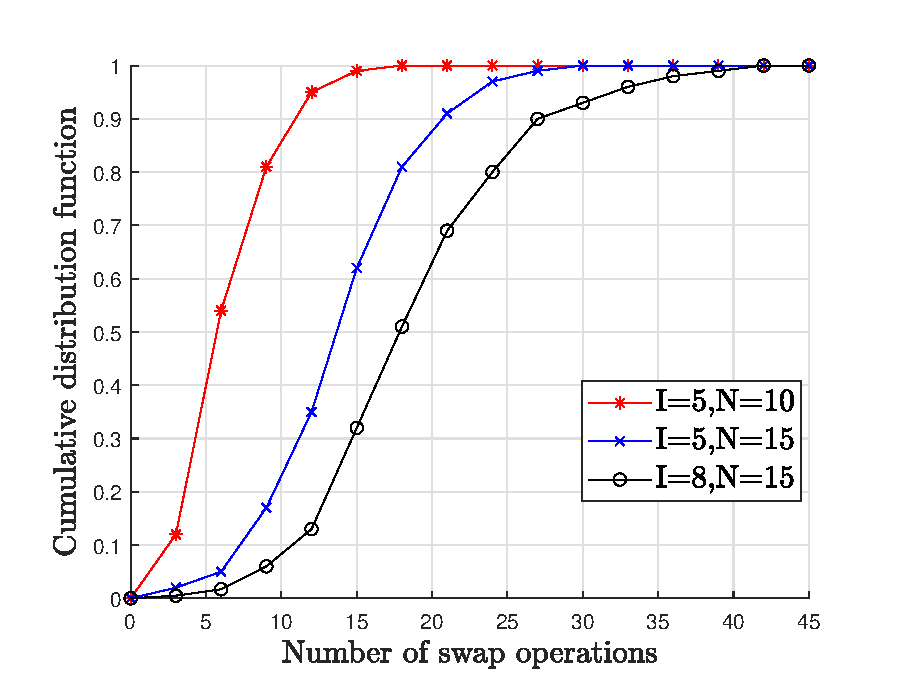
\includegraphics[width=0.6\textwidth]{figs_tvt_cld/Figure3b.eps}\label{4-2}}
	\subfigure[t=1.2 ms]{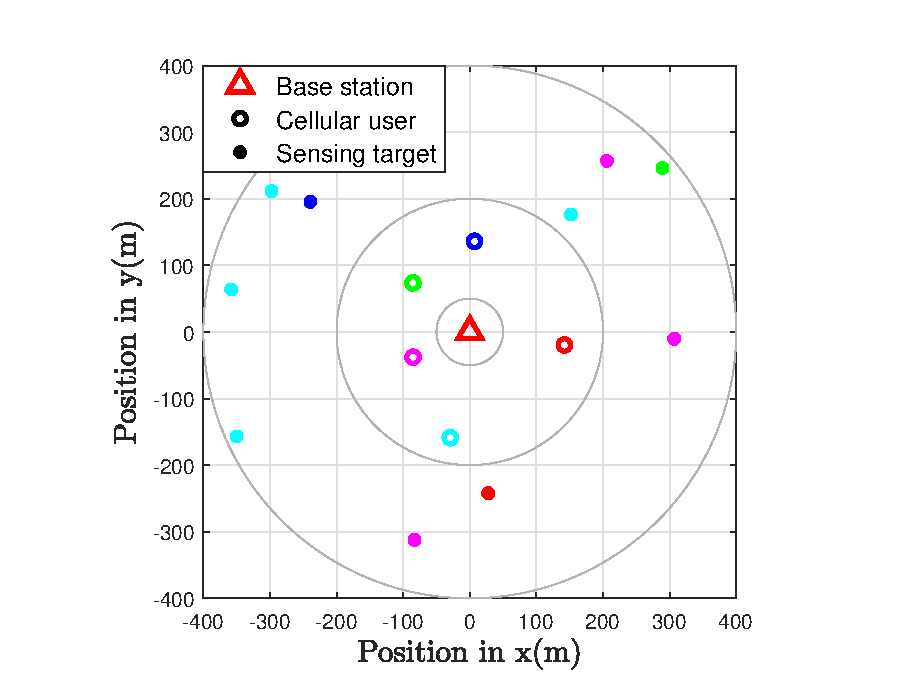
\includegraphics[width=0.6\textwidth]{figs_tvt_cld/Figure3c.eps}\label{4-3}}
	\caption{Convergence of Algorithm 5 under $K=4$ and $M=3$}
	\label{fig:Con_2-1}
\end{figure*}
\begin{figure*}
	\centering
	\subfigure[t=1.5 ms]{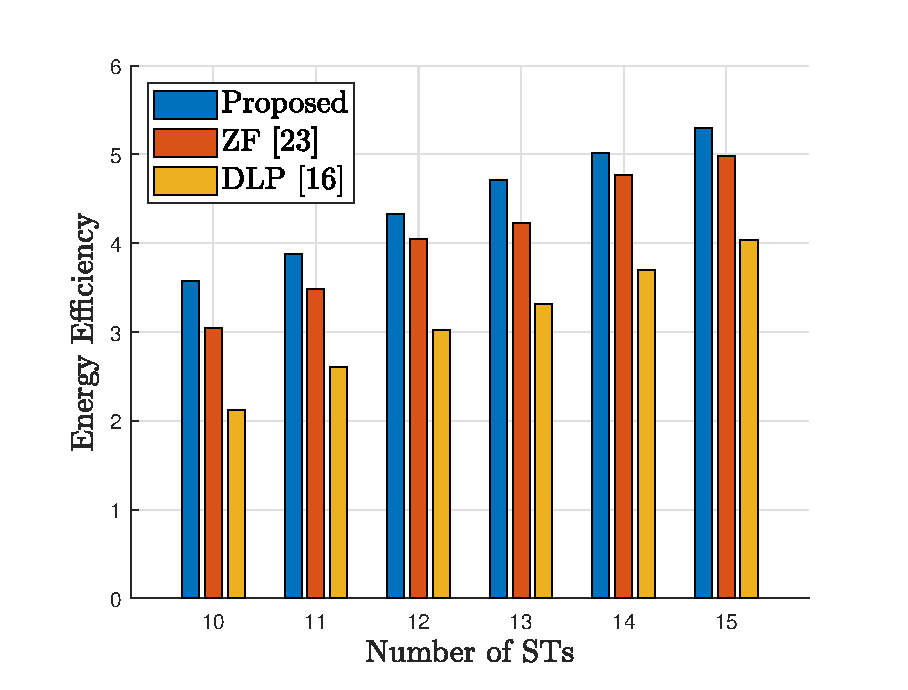
\includegraphics[width=0.6\textwidth]{figs_tvt_cld/Figure4a.eps}\label{4-4}}
	\subfigure[t=1.82 ms]{\includegraphics[width=0.6\textwidth]{figs_tvt_cld/Figure4b.eps}\label{4-5}}
	\subfigure[t=2.0 ms]{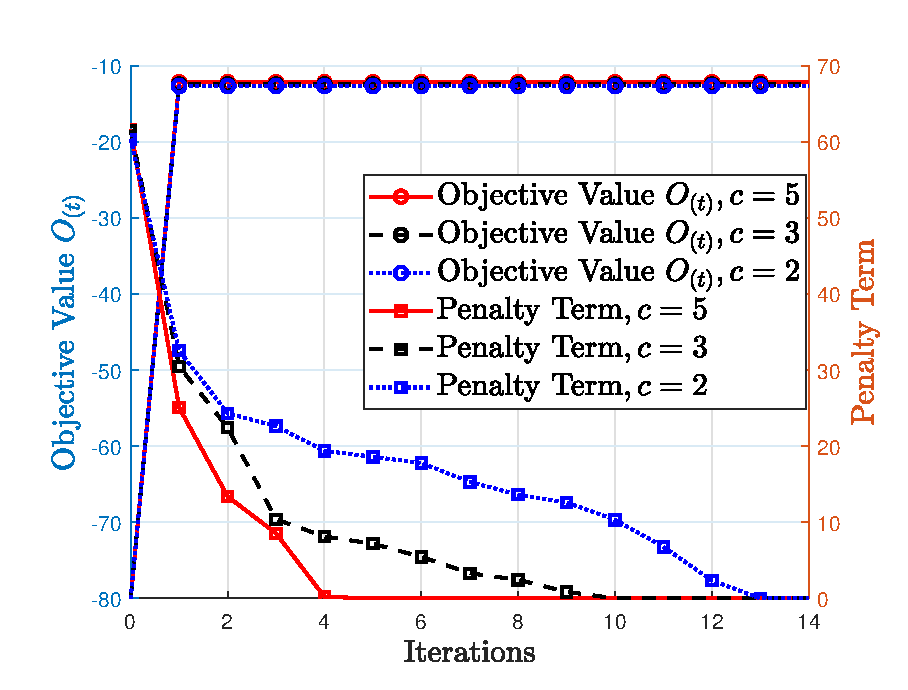
\includegraphics[width=0.6\textwidth]{figs_tvt_cld/Figure4c.eps}\label{4-6}}
	\caption{Convergence of Algorithm 5 under $K=4$ and $M=6$}
	\label{fig:Con_2-2}
\end{figure*}
In this section, numerical results are provided to verify the effectiveness of our algorithms and to show the performance of our NOMA-aided ISAC system. Specifically, we assume that the ISAC BS is equipped with a uniform linear array of 4-antennas. The ISAC BS requires to serve $M=3$ or $6$ NUs while performing sensing towards a group of $I=5$ STs. The NUs are randomly distributed within a radius of $d_m\in[50,200]~m$ from the center of the ISAC BS, and the STs are evenly distributed within a radius of $d_i\in[200,300]~m$ to centered on the ISAC BS. We assume that the amount of tasks required by the NUs arrives randomly between $[5,10]~MB$, and directions $\{\theta_i\}_{i\in\mathcal{I}}$ of five STs are $\theta_1=-60^\circ$, $\theta_2=-30^\circ$, $\theta_3=0^\circ$, $\theta_4=30^\circ$ and $\theta_5=60^\circ$. The total power capacity is $P^{\text{max}}=20~dBm$, the channel bandwidth is $B=8~MHz$, and the noise power is $\sigma_n^2=-110~dBm$. In addition, the channel between the ISAC BS and NUs is considered to follow the Rayleigh channel model with the path loss of $\sqrt{\beta_m}=40+30\log_{10}d_m$, while the channel between the ISAC BS and STs is supposed to have a line-of-sight (LoS) link correlated with the path loss of $\sqrt{\mu_i}=40+25\log_{10}d_i$. To characterize the channel spatial correlations of the NUs, based on \cite{tvt.kermoal2002stochastic}, we model the channel gains as 
\begin{eqnarray}
	\mathbf{G}\triangleq\left[\frac{\mathbf{g}_1}{||\mathbf{g}_1||},\frac{\mathbf{g}_2}{||\mathbf{g}_2||},...,\frac{\mathbf{g}_I}{||\mathbf{g}_I||}\right]=\tilde{\mathbf{G}}\mathbf{C}_{\mathbf{G}}^{1/2},
	\label{spatial}
\end{eqnarray}
where $\tilde{\mathbf{G}}$ denotes the normalized Rayleigh fading matrix and satisfies $\mathbb{E}\left[\tilde{\mathbf{G}}^H\tilde{\mathbf{G}}\right]=\mathbf{I}$. $\mathbf{C}_{\mathbf{G}}$ represents the covariance of $\mathbf{G}$, where the $(m,n)$-th factor indicates the channel relevance of NU $m$ and NU $n$ with the norm of $\tau^{|m-n|}$. Finally, the convergence thresholds of Algorithm 4 and Algorithm 5 are set to $\vartheta=10^{-5}$ and $\Delta=10^{-5}$.






Figures \ref{fig:Con_2-1} and \ref{fig:Con_2-2} validate the convergence and effectiveness of our Algorithm 5 under different settings. Specifically, it can be observed that for arbitrary value of the coefficient $c$, the objective value can converge rapidly and the penalty term can also converge almost to zero after a few iterations. It can also be seen from Figure 3.4(b) that the convergence speed increases when the value of the coefficient $c$ increases. However, an increase in $c$ will degrade the objective function, i.e., $O_{(t)}$ becomes larger. Such a result indicates a trade-off between the convergence speed and computation accuracy of Algorithm 5. In addition, Figures 3.3 and 3.4 show that the output of the Subroutine-O is almost zero when the value of $t$ is optimal, which also verifies the correctness of Proposition 5 and Algorithm 4.




Figure \ref{fig:Con_1} verifies the convergence of our Algorithm 4 under given $\{x_i\}_{i\in\mathcal{I}}$. Under two tested cases of $K=4,~M=3$ and $K=4,~M=6$, the top sub-figure of Figure \ref{fig:Con_1} displays the value of $O_{(t)}$ for the output of Subroutine-O (i.e., Algorithm 5), and the bottom sub-figure displays the convergence of NOMA transmission duration $t$. We mark out the final convergence to the values in the two subplots with the red dashed lines. As expected, the value of $t$ converges to the optimal value $t^*$ when $O_{(t)}$ is close to zero. Moreover, we can observed that when $t$ increases, the value of $O_{(t)}$ is non-increasing, which verifies the Proposition 5.




Figure \ref{fig:Con_3} shows the convergence of Algorithm 6 and the conventional CE scheme. With the convergence values in Figure 6, we can obtain the optimal sensing scheduling, in this case, $\{x_i\}=\{0,1,1,1,0\}$, for the current setup. It can be observed that with the introduced probability update strategy, our proposed CE learning based algorithm performs a less number of iterations than the conventional CE scheme. 



\begin{figure}
	\centering
	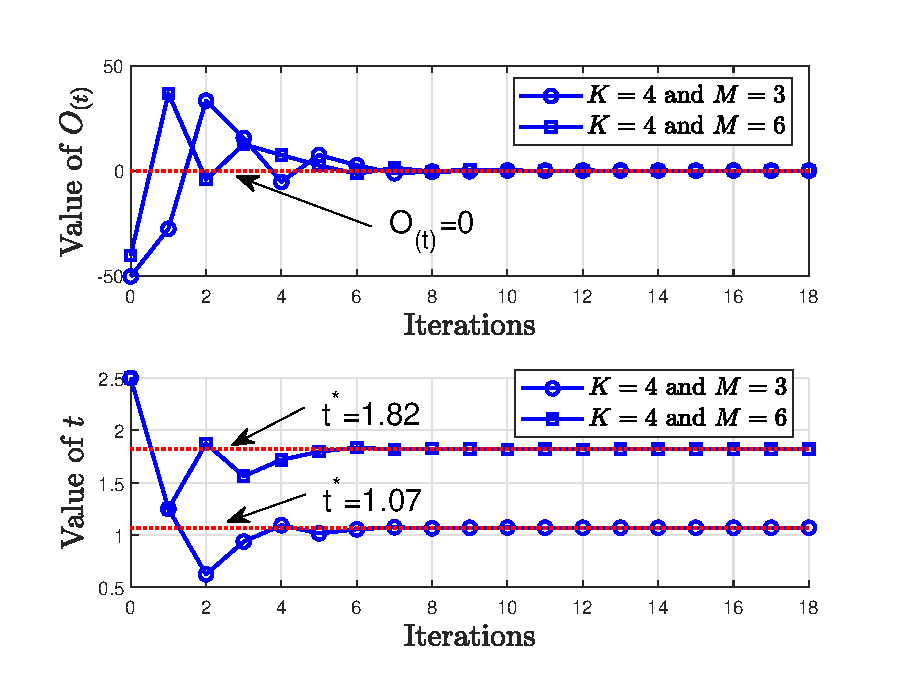
\includegraphics[width=0.6\textwidth]{figs_tvt_cld/Figure5.eps}
	\caption{Convergence of Algorithm 4}
	\label{fig:Con_1}
\end{figure}
\begin{figure}
	\centering
	\subfigure[Proposed CE scheme]{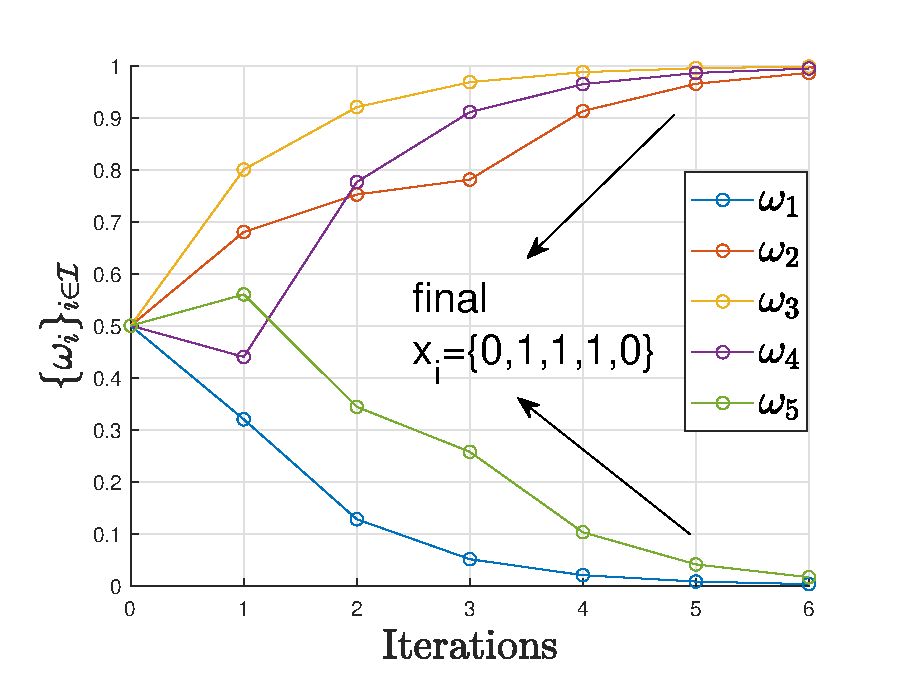
\includegraphics[width=0.48\textwidth]{figs_tvt_cld/Figure6a.eps}\label{6-1}}
	\subfigure[Conventional CE scheme]{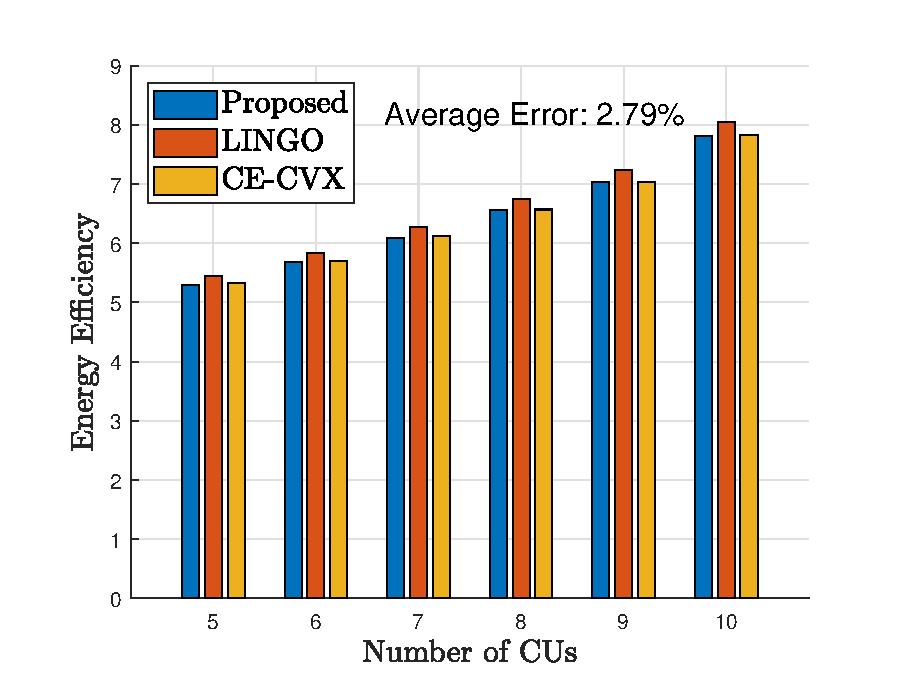
\includegraphics[width=0.48\textwidth]{figs_tvt_cld/Figure6b.eps}\label{6-2}}
	\caption{Convergence of Algorithm 6 under $K=4$ and $M=3$}
	\label{fig:Con_3}
\end{figure}
\begin{figure*}
	\centering
	\subfigure[Comparison of sensing efficiency]{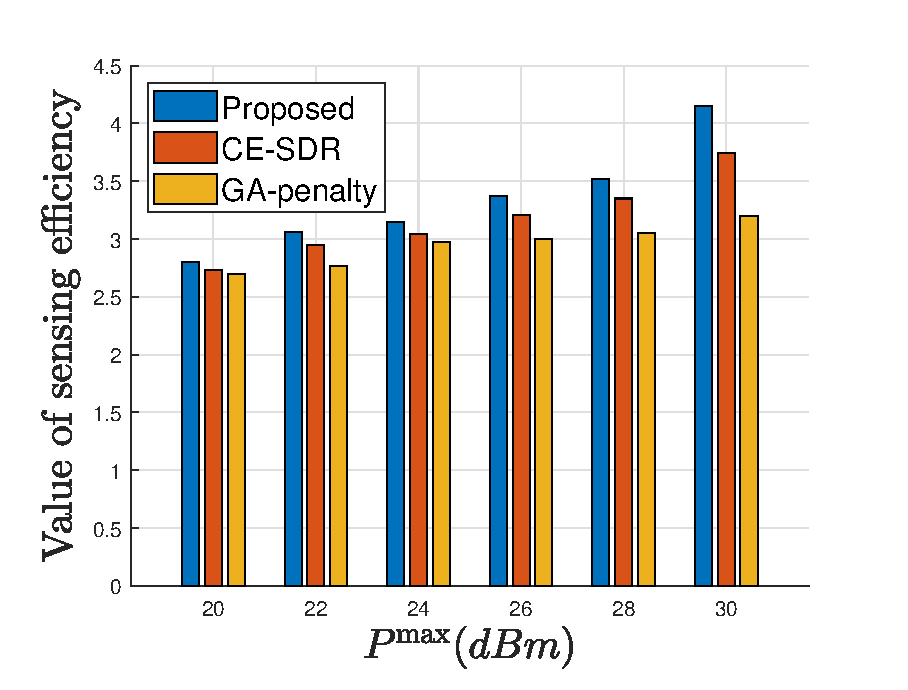
\includegraphics[width=0.6\textwidth]{figs_tvt_cld/Figure7a.eps}\label{9-1}}
	\subfigure[Comparison of total throughput]{\includegraphics[width=0.6\textwidth]{figs_tvt_cld/Figure7b.eps}\label{9-2}}
	\subfigure[Comparison of computation time]{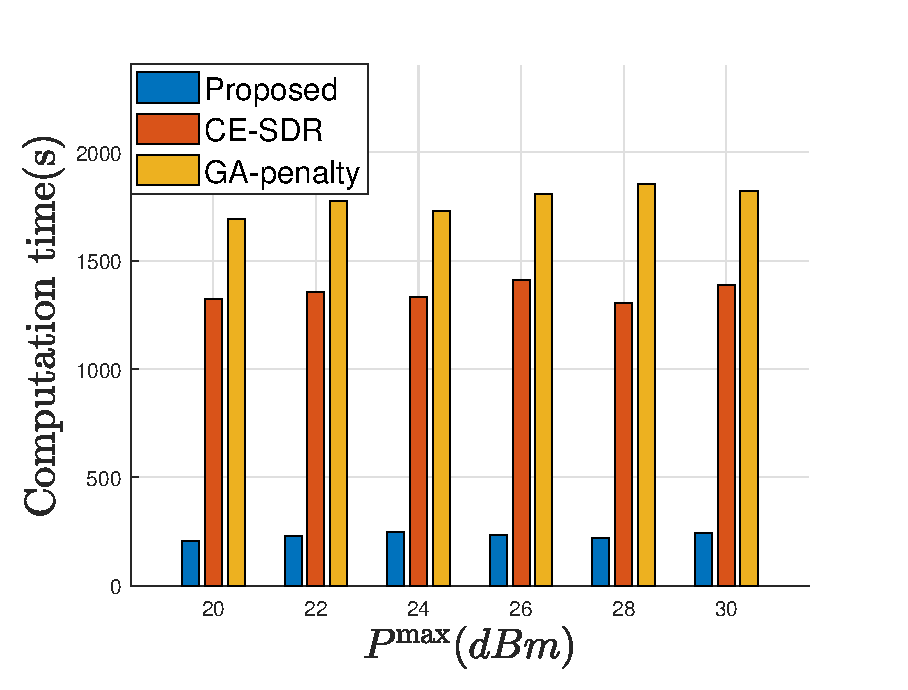
\includegraphics[width=0.6\textwidth]{figs_tvt_cld/Figure7c.eps}\label{9-3}}
	\caption{Performance advantages of our proposed algorithm compared with benchmark algorithms}
	\label{fig:Compare-algorithms}
\end{figure*}



Figure \ref{fig:Compare-algorithms} shows the performance of our algorithm in terms of sensing efficiency, total throughput and computation time compared with some benchmark algorithms. Specifically, we set $K=4$ and $N=3$ and use the following two algorithms as the comparison benchmarks.
\begin{itemize}
	\item CE-SDR algorithm. We utilize the CE learning based algorithm proposed in this chapter to solve Problem (SEM-E-Top), and utilize the method of semidefinite relaxation (SDR) and Gaussian randomization to solve Problem (SEM-E-BOT) \cite{tvt.luo2010semidefinite}.
	\item GA-penalty algorithm. We utilize genetic algorithm (GA) to solve Problem (SEM-E-Top) \cite{tvt.holland1992genetic}, and utilize penalty-based method proposed in this chapter to solve Problem (SEM-E-BOT).
\end{itemize}
Figure \ref{fig:Compare-algorithms} shows that our algorithm outperforms the benchmark algorithms in all three aspects. In particular, the algorithm proposed in this chapter significantly outperforms the other two benchmark algorithms in terms of computation time. In addition, when the total power capacity $P^{\text{max}}$ increases, the sensing efficiency and the total throughput increase accordingly. 







Figure \ref{fig:Performance} demonstrates the communication performance, i.e., total throughput, with different spatial correlation under $t^*$. Each point in Figure \ref{fig:Performance} represents the average result of 200 random channel realizations. We compare the achievable communication capability  of our NOMA-aided ISAC with the conventional ISAC and use the communication-only (CO) scheme as an upper bound for the communication performance. Specifically, the achievable rate at communication user $\forall m\in\mathcal{M}$ in the conventional ISAC can be expressed as
\begin{eqnarray}
	R_{m,\text{con}}=B\log_2\left(1+\frac{|\mathbf{g}_m^H\mathbf{w}_m|^2}{\sum\limits_{n\in\mathcal{M},n\neq m}|\mathbf{g}_m^H\mathbf{w}_n|^2+\sigma_n^2}\right).
	\label{CISAC}
\end{eqnarray}
It can be observed that the achievable communication performance of NOMA-aided ISAC is almost independent of the channel spatial correlation, while the achievable communication performance of conventional ISAC degrades severely as the channel spatial correlation increases. 

\begin{figure}
	\centering
	\subfigure[$K=4$ and $M=3$]{\includegraphics[width=0.48\textwidth]{figs_tvt_cld/Figure8a.eps}\label{7-1}}
	\subfigure[$K=4$ and $M=6$]{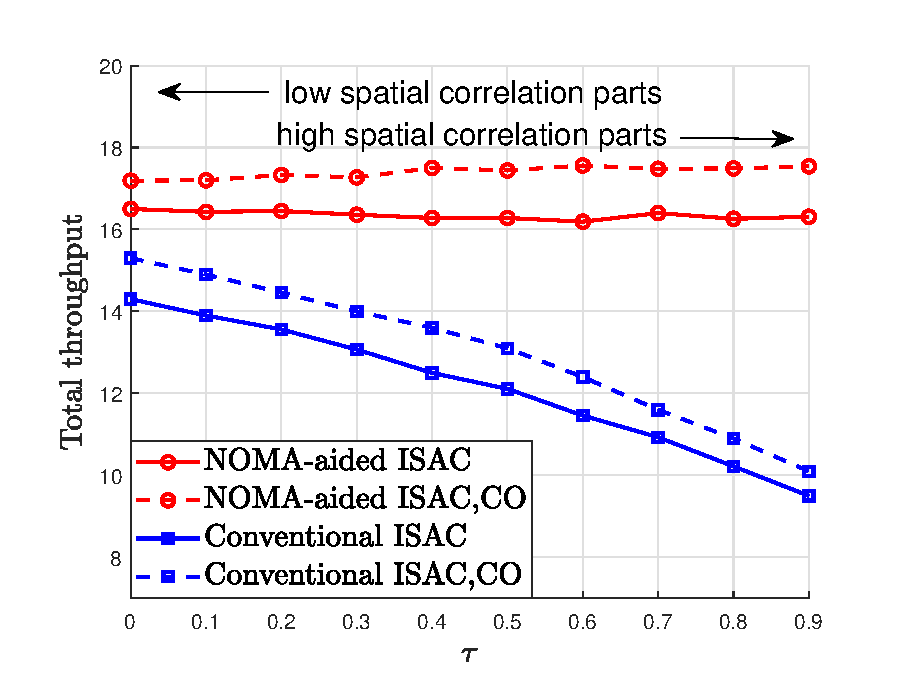
\includegraphics[width=0.48\textwidth]{figs_tvt_cld/Figure8b.eps}\label{7-2}}
	\caption{Communication performance with different $\tau$ under $t^*$}
	\label{fig:Performance}
\end{figure}


We consider in Figure \ref{fig:Performance}(a) the case of the number of antennas $K=4$ and the number of NUs $M=3$. As can be observed from Figure \ref{fig:Performance}(a) that the NOMA-aided ISAC achieves better communication performance at high channel spatial correlation. This is because under high channel spatial correlation, the spatial DoFs are restricted, while NOMA can provide additional DoFs to ensure the communication capability. In Figure \ref{fig:Performance}(b), we consider the case of $K=4$ and $M=6$, in which it is not possible to assign one spatial DoF to each NU, in spite of not performing sensing. As we can see from Figure \ref{fig:Performance}(b), there is a significant loss in the communication performance achieved because conventional ISAC cannot mitigate inter-user interference well and require sacrificing a portion of communication resources to guarantee the sensing performance. The NOMA-aided ISAC outperforms the conventional ISAC in terms of the communication capability, regardless of the strength of channel spatial correlation. This is because the NOMA-aided ISAC can still provide additional DoF by mitigating inter-user interference through SIC. In addition, the NOMA-aided ISAC is closer to the upper limit of achievable communication performance in the communication-only scheme than conventional ISAC.

\begin{figure}
	\centering
	\subfigure[$K=4$ and $M=3$]{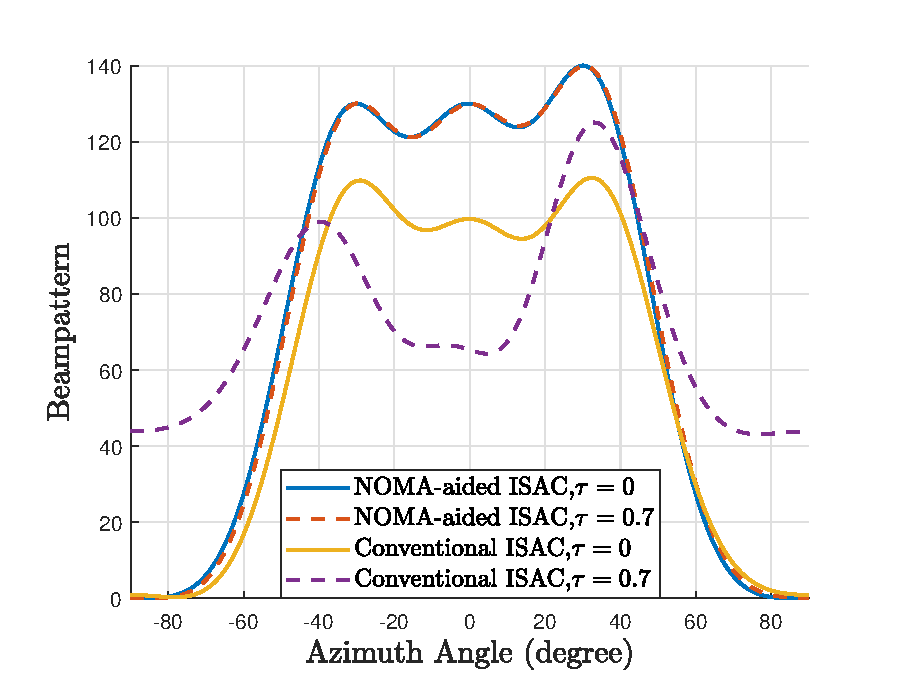
\includegraphics[width=0.48\textwidth]{figs_tvt_cld/Figure9a.eps}\label{8-1}}
	\subfigure[$K=4$ and $M=6$]{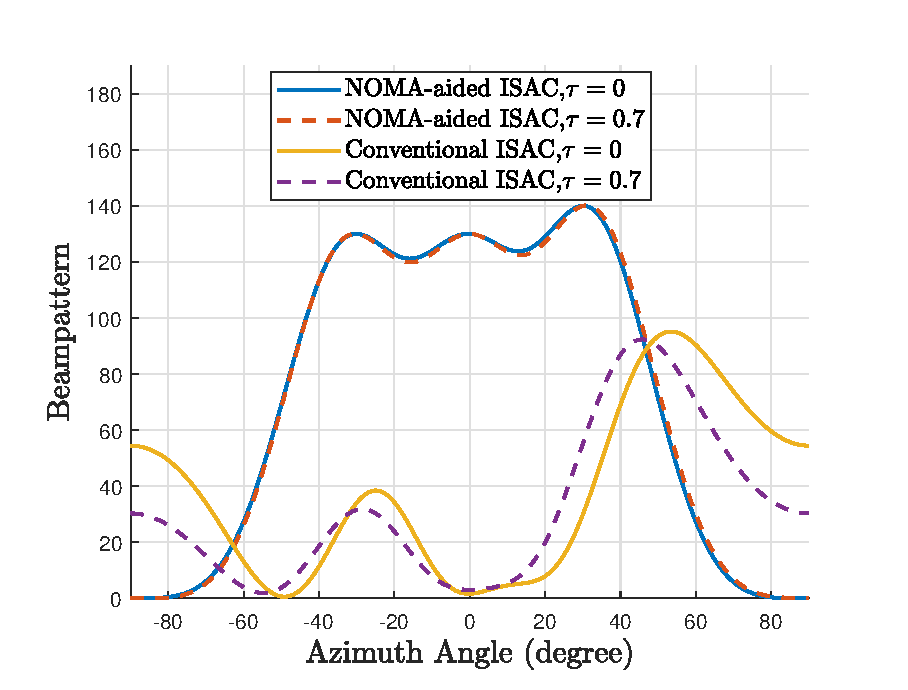
\includegraphics[width=0.48\textwidth]{figs_tvt_cld/Figure9b.eps}\label{8-2}}
	\caption{Transmit beampattern}
	\label{fig:beampattern}
\end{figure}


\begin{figure*}
	\centering
	\subfigure[Comparison of sensing efficiency]{\includegraphics[width=0.6\textwidth]{figs_tvt_cld/Figure10a.eps}\label{10-1}}
	\subfigure[Comparison of total throughput]{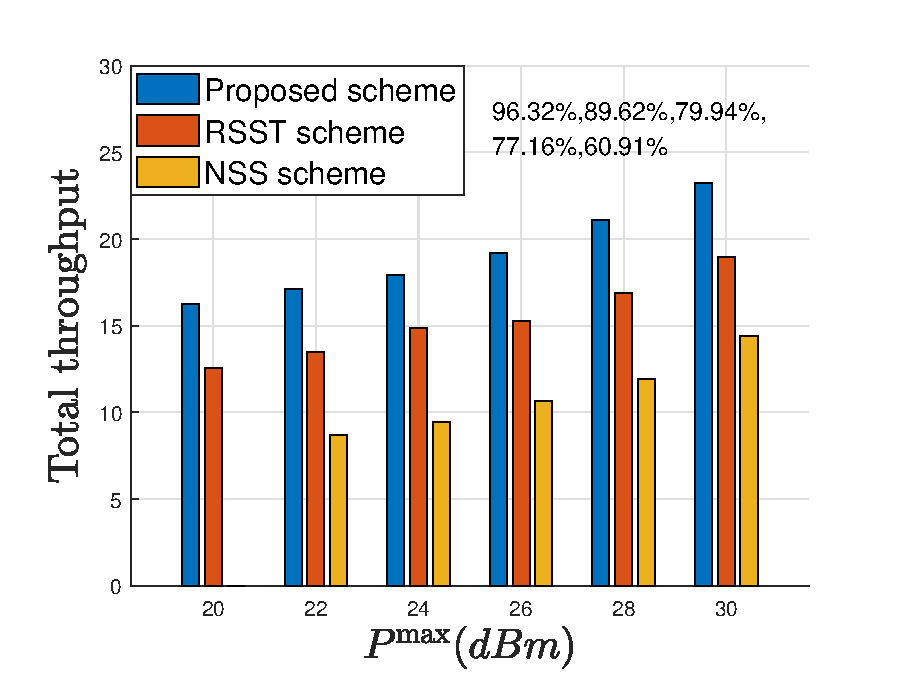
\includegraphics[width=0.6\textwidth]{figs_tvt_cld/Figure10b.eps}\label{10-2}}
	\subfigure[Comparison of NOMA transmission duration]{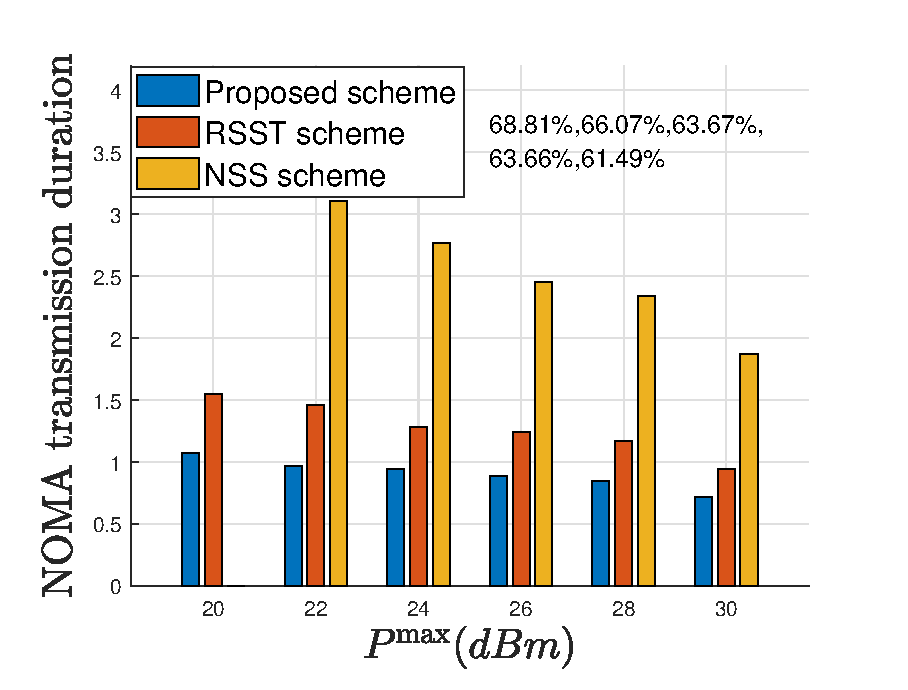
\includegraphics[width=0.6\textwidth]{figs_tvt_cld/Figure10c.eps}\label{10-3}}
	\caption{Performance advantages of our proposed algorithm compared with benchmark schemes}
	\label{fig:Compare-schemes}
\end{figure*}


Figure \ref{fig:beampattern} compares the transmit beampatterns of NOMA-aided ISAC and conventional ISAC with different channel spatial correlations. As can be observed from Figure \ref{fig:beampattern}(a) that at low spatial correlation, both schemes are capable of realizing the dominant peak of the transmitted beampattern in the direction of interest, and at high spatial correlation, the power gain of the conventional ISAC in the above direction is significantly reduced. When the number of NUs increases, in Figure \ref{fig:beampattern}(b), the NOMA-aided ISAC can still achieve dominant peaks, while the conventional ISAC has major damage to power leakage in undesirable directions. 


Figure \ref{fig:Compare-schemes} shows the advantages of the proposed sensing scheduling scheme in comparison with the random selection of sensing targets (RSST) scheme and the no-sensing scheduling (NSS) scheme. Figure \ref{fig:Compare-schemes} shows that the sensing scheduling scheme proposed in this chapter outperforms the other two schemes in terms of both communication and sensing performance. In particular, the gain obtained by our sensing scheduling scheme over the scheme without accounting for the sensing scheduling (i.e., NSS scheme) is marked at the top of three subplots. Moreover, it can be observed from the first set of data in each of the subplots of Figure \ref{fig:Compare-schemes} that when sensing scheduling is not considered, sensing may even fail to execute (i.e., failing to reach the sensing requirements for any of the STs). This further illustrates the importance of sensing scheduling.


\section{Conclusion} \label{chap3_sec_conclusion}
In this chapter, we have investigated the NOMA-aided ISAC system. Specifically, we have utilized the superimposed NOMA signal for the NUs to perform multi-target sensing while satisfying the quality of service for both communication and sensing. We have proposed a joint optimization of the beamforming, the NOMA transmission duration and the sensing scheduling, with the objective of maximizing the sensing efficiency in ISAC system. Despite the formulated joint optimization problem is strictly non-convex, we have exploited the vertical layered structure of the problem and proposed a decomposition-based algorithm that employs the techniques of the penalty function and SCA and the CE learning. Numerical results have been provided to validate the effectiveness of our algorithms and the performance benefits of the proposed NOMA-aided ISAC sensing scheduling scheme.
